\chapter{Literature Review}
\section{\acrlong{llm}}
Some LLMs that will be discussed in this section:

\begin{itemize}
\item{Gemma 3}
\item{DeepSeek R1}
\item{Mixtral}
\item{Qwen}
\end{itemize}

\paragraph{} The paper \textcite{deepseek-ai_deepseek-r1_2025} tells us about DeepSeek's R1-Zero and  R1 models. In particular it says that the models are based on the existing DeepSeek V3 MoE model, but have been further trained to allow for \acrfull{cot} reasoning similar to ChatGPT's O1. ChatGPT O1 is one of the first \acrshort{cot} models and is closed source. R1-Zero was created by applying reinforcement learning to the V3 model, which was successful in producing a model with \acrshort{cot} capabilities. It did however have problems such as language mixing. To deal with these issues another model was created, called R1. R1 used both reinforcement learning like R1-Zero, but also used supervised fine tuning with a small amount of cold-start data. This lead to a model without the issues seen in R1-Zero. The paper also covers a technique called distillation: this is where a larger model like R1 is used to train smaller models. In this case distillation was used to train multiple \acrshort{llama} and Qwen base models to have Chain of Thought capabilities. This technique was compared against doing reinforcement learning directly on the \acrshort{llama} and Qwen models to create Chain of Thought reasoning. It was found that the distillation technique resulted in more effective models. Both the full model and the distilled models have been open-sourced.

\paragraph{}Qwen have a series of models they have released. One of these is a reasoning model called qwq. According to their benchmarks from \textcite{} it has performance comparable to the full 671 billion parameter DeepSeek R1 despite only being 32 billion parameters in size. It also compares favorably to OpenAI's o1-mini and the smaller distilled versions of DeepSeek R1. These benchmarks are shown in a copy of their graph in figure \ref{fig:qwq-performance}.

\begin{figure}
    \centering
    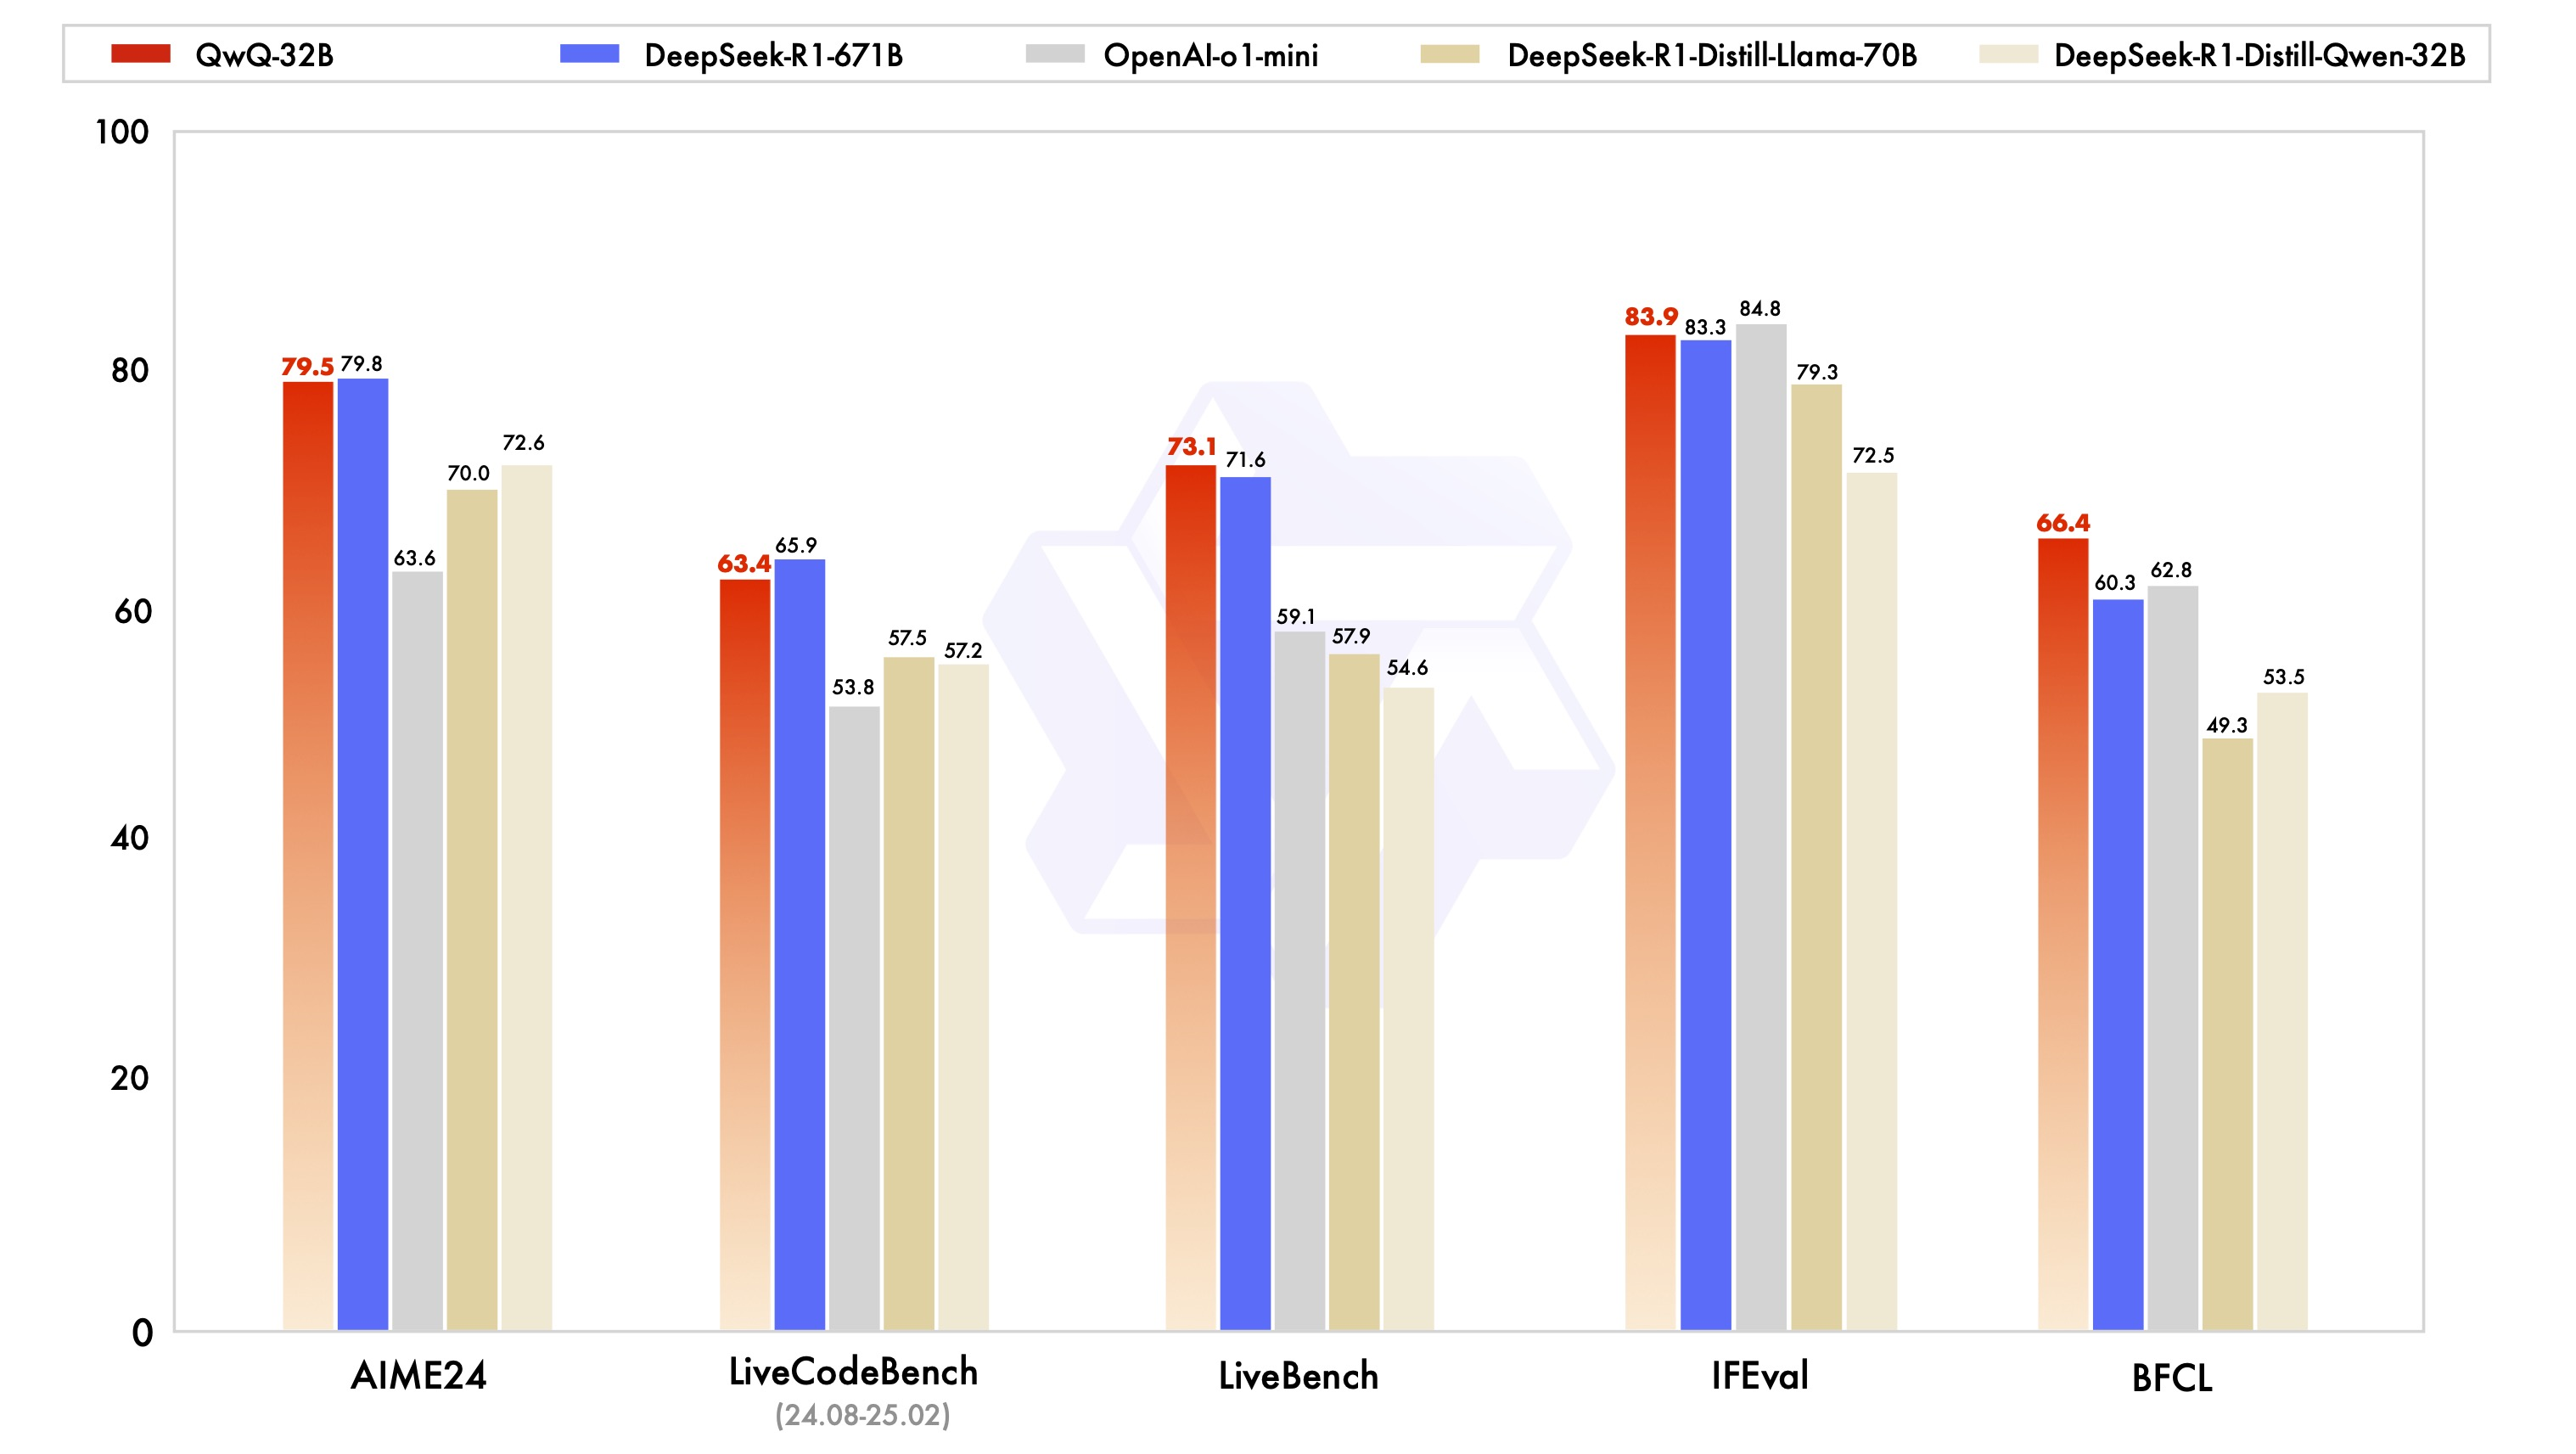
\includegraphics[width=1\linewidth]{figure/qwq-32b-final.jpg}
    \caption{QwQ performance in benchmarks}
    \label{fig:qwq-performance}
\end{figure}

\paragraph{}\autocite{chen_parallel_2025} is a paper exploring a new way of improving \acrshort{llm} performance through a new kind of scaling rule. Rather than using parameter scaling (making larger dense or MoE models), or inference time scaling (reasoning models), this instead uses one set of parameters being executed in parallel and the results combined together. By creating a model using this method, they were able to come up with something that requires a fraction of the memory than a similar performing dense model while having improved lantecy. Table \ref{tab:compare} is a copy of the table from this paper showing the advantages and disadvantages of different LLM scaling methods.



%Table from study
{
\begin{table}[t]
\caption{Copy of comparison table from \textcite{chen_parallel_2025}}
\centering
\resizebox{\linewidth}{!}{
\begin{tabular}{lllll}
\toprule
Method & Inference Time & Inference Space & Training Cost & Specialized Strategy \\
\midrule
Dense Scaling &  \emoji{figure/neutral_face} Moderate & \emoji{figure/rage} High & \emoji{figure/rage} Pre-training only & \emoji{figure/grin} No \\
MoE Scaling & \emoji{figure/grin} Low & \emoji{figure/rage} High & \emoji{figure/rage} Pre-training only & \emoji{figure/rage} \makecell[l]{Load balancing} \\
\makecell[l]{Inference-Time Scaling} & \emoji{figure/rage} High & \emoji{figure/neutral_face} Moderate & \emoji{figure/grin} \makecell[l]{Post-training} & \emoji{figure/rage} \makecell[l]{RL / reward data} \\
Parallel Scaling & \emoji{figure/neutral_face} Moderate & \emoji{figure/neutral_face} Moderate & \emoji{figure/grin} \makecell[l]{Pre- or Post-training} & \emoji{figure/grin} No \\
\bottomrule
\end{tabular}
}
\label{tab:compare}
\end{table}
}

\section{Image generation models}
\paragraph{}






\section{Fine Tuning models}

\section{\acrfull{rag}}
\acrshort{rag} is a technique that allows an LLM to access external data. This is done by having the LLM send the data to another model. This is converted to an embedding/vector. The embedding model uses this to search through a index of a knowledge base. This index also contains vectors that are compared against the vectors of the query. The retrieved information if then sent back to the LLM to generate a response. \acrshort{rag} could be used in a variety of applications including helping lawyers, doctors, and financial analysts with questions. \autocite{merritt_what_2025}.

\section{Agentic \acrshort{ai}}
\paragraph{}Agentic AI is capable of goal-oriented, autonomous action and is adaptable. These AIs are based on generative AI such as LLMs. Unlike conventional LLMs they are not limited to the information they are trained on as they can do things such as independently gather new information. Like an LLM an agentic AI can be interacted with through a natural language prompt, making them simpler to use than other software products. \autocite{noauthor_what_2025}.

\paragraph{}According to \textcite{pounds_what_2024} agentic AI uses a four step process:
\begin{enumerate}
    \item Perceive
    \item Reason
    \item Act
    \item Learn
\end{enumerate}

\paragraph{}The last step called learn involves gathering data from the system in use, and using it to train future iterations of the model. This creates a feedback loop called the data flywheel.

\section{\acrshort{ai} in Scenario Generation}

\paragraph{}

\section{Character \acrshort{ai} and chatbots}